%% IEEE conference paper. Every sentence that contains a number sits on its own line and ends
%% with a comment naming its evidence row in paper/EVIDENCE.md (see paper/STYLE_GUIDE.md).
%% Tables and figures are generated by paper/ieee/scripts/make_tables.py and make_figures.py.
\documentclass[conference]{IEEEtran}
\usepackage{cite}
\usepackage{amsmath,amssymb}
\usepackage{graphicx}
\usepackage{booktabs}
\usepackage{url}

\hyphenation{epi-demi-o-log-i-cal}

\begin{document}

\title{SEIR-Informed Graph Learning for Weekly Dengue Forecasting: A Development Evaluation Against Persistence}

% Venue: ICITR, University of Moratuwa. User-specified maximum: 6 pages including references.
\author{\IEEEauthorblockN{Tharusha Perera, Praveen De Silva, Janith Mahanama,\\
Bimsara Udurawana, Maleesha Kumarasinghe, Praveen Nawarathna}
\IEEEauthorblockA{Department of Computer Science and Engineering, University of Moratuwa\\
Moratuwa, Sri Lanka\\
\{tharushap.23, praveend.23, janithm.23, bimsarau.23,\\
kumarasinghemp.23, praveenn.23\}@cse.mrt.ac.lk}}

\maketitle

\begin{abstract}
Graph neural networks and epidemic compartment models offer different ways to represent district-level dengue dynamics.
We evaluate their forecasting behavior against persistence, which repeats the latest reported count.
The rebuilt dataset contains 559 reporting weeks for 25 Sri Lankan districts, with missing reports retained as missing. % EV-163
We compare static and adaptive graph encoders with direct, residual, and susceptible--exposed--infectious--recovered (SEIR) output heads.
The existing evaluations are development evidence: earlier test periods informed later model choices, and the stored runs precede a correction to the geographic graph.
Forecast targets also overlap at partition boundaries.
Across nine rolling origins, persistence has a test root mean squared error of 28.54 cases per district-week, compared with 27.45 for the anchored adaptive SEIR model. % EV-100, EV-114
Its paired difference is -1.10 cases, with a descriptive 95\% interval from -2.84 to +0.65; the Benjamini--Hochberg adjusted test value is 0.576. % EV-215, EV-114
The interval does not establish equivalence or an improvement.
Exploratory output-head comparisons suggest that a persistence anchor accounts for much of the validation improvement in poorly fitted direct-head models, while test results favor the SEIR versions.
These comparisons lack equal validation-only tuning and do not isolate the epidemic equations on the adaptive encoder.
Corrected-data reruns, classical baselines, and an untouched-period evaluation remain necessary before a confirmatory claim.
\end{abstract}

\begin{IEEEkeywords}
dengue forecasting, graph neural networks, persistence baseline, physics-informed learning, rolling-origin evaluation, SEIR model
\end{IEEEkeywords}

%=====================================================================
\section{Introduction}
Dengue is a mosquito-borne disease that causes recurring epidemics in Sri Lanka~\cite{tissera2020severe}.
Forecasts of weekly cases for each district, a few weeks ahead, could help health officers decide where to place clinical capacity and vector control.
Graph neural networks model exchange between neighboring districts, and epidemic compartment models encode how infection spreads.
Prior work studies graph forecasting and epidemiologically informed prediction~\cite{weng2024graph,gulmohamed2026denguegnn,rodriguez2023einns,wang2022causalgnn,cao2023mepognn,liu2025seirlstm}.

A forecast is useful only if it beats a trivial baseline.
For weekly counts, the trivial baseline is persistence: repeat last week's value.
The pooled squared correlation between consecutive weekly counts is 0.8893. % EV-004
This describes association across district-weeks, rather than out-of-sample forecast skill.
The benchmark paper for this dataset reports no persistence baseline~\cite{weng2024graph}.
Two further issues affect the interpretation of our benchmark comparisons.
The widely used data array contains one week that is wrong because of a formula error in the source table, and persistence scores 44.80 with that week and 29.52 without it. % EV-006
Studies with few forecast origins also cannot produce small $p$-values: an exact sign-flip test on three origins cannot return $p$ below 0.25. % EV-181

We therefore ask a narrow question.
We assess whether this SEIR-informed architecture improves forecasts relative to persistence.
The stored results are development evidence, and they motivate a corrected-data evaluation before any confirmatory conclusion.
Our contributions are as follows.
\begin{enumerate}
\item A source audit identifying a published table error and its effect on the persistence baseline (Section~\ref{sec:data}).
\item A development comparison of graph encoders and output heads, with paired differences and uncertainty reported alongside persistence (Section~\ref{sec:results}).
\item An analysis of the distinction between persistence anchoring and SEIR decoding, including missing controls and mixed validation/test findings (Section~\ref{sec:discussion}).
\end{enumerate}

%=====================================================================
\section{Related Work}
Weng et al.~\cite{weng2024graph} benchmark adapted encoders on Sri Lankan dengue counts.
These include spatial-temporal graph attention (STGAT)~\cite{huang2019stgat} and attention temporal graph convolution (A3T-GCN)~\cite{bai2021a3tgcn}.
They also evaluate attention-based spatial-temporal graph convolution (ASTGCN)~\cite{guo2019astgcn}, diffusion convolutional recurrence (DCRNN)~\cite{li2018dcrnn}, and adaptive graph convolution (AAGCN)~\cite{shi2019aagcn}.
Their comparison set has no naive baseline.
DengueGNN~\cite{gulmohamed2026denguegnn} builds a dynamic adjacency from an assumed gravity-mobility law and adds no mechanistic constraint.
Graph WaveNet~\cite{wu2019graphwavenet} supplies the adaptive adjacency that we reuse.

Several epidemic models place mechanistic structure inside a neural network.
Liu et al.~\cite{liu2025seirlstm} let an LSTM output the force of infection of an SEIR model for Sri Lankan dengue, which is the design our SEIR heads follow with graph encoders.
EINNs~\cite{rodriguez2023einns}, CausalGNN~\cite{wang2022causalgnn} and MepoGNN~\cite{cao2023mepognn} add epidemiological structure to graph or recurrent models.
We use a human-only SEIR model, as Liu et al. do; explicit host-vector compartments are omitted.
Physics-informed losses~\cite{raissi2019pinn} can fail to train when the constraint is hard to satisfy~\cite{krishnapriyan2021failure}.

Interval coverage must be interpreted together with interval width~\cite{bracher2021evaluating}.

%=====================================================================
\section{Data and Problem Setup}\label{sec:data}
We forecast weekly dengue notifications for the 25 districts of Sri Lanka. % EV-216
We rebuilt the series from the original weekly epidemiological reports.
The rebuilt series has 559 weeks, of which 7 have no report; we leave them missing and never interpolate. % EV-163
Any forecast window whose case inputs or targets touch a missing report is dropped.
The verified report calendar runs from June 15, 2013, to February 24, 2024. % EV-216
These are report dates rather than ISO week labels.
The source-series visualization is provided in the supplementary material.

An earlier benchmark array, which we call the legacy array, has 459 weeks~\cite{weng2024graph}. % EV-002
In it, the national total is 7165 cases in week 395, against 396 and 414 in the weeks on either side. % EV-162
The jump is not a real surge.
The corresponding published table contains internally inconsistent district and national totals~\cite{epid2021wer0248}; source checks identify a spreadsheet formula error.
Persistence has an RMSE of 44.80 on the legacy array and 29.52 once that week is excluded. % EV-006
We use the legacy array only in Section~\ref{sec:results} to label older results.

Case inputs are lagged one week; the stored nine-origin encoders use case histories only. % EV-003, EV-179
SEIR heads additionally use population and initial compartment fractions.
Date-dependent covariate comparisons await replacement and are excluded from the main claims.

The task is to map 3 weeks of counts for all districts to the next 3 weeks, which gives horizons $h=1,2,3$. % EV-007
Districts are graph nodes, and the static graph is intended to represent shared borders.
The historical file also contains two directed edges that are not borders. % EV-010
The graph has 25 nodes and 141 directed edges including self-loops. % EV-010

%=====================================================================
\section{Methods}\label{sec:methods}
Fig.~\ref{fig:arch} summarizes the models.
Each neural model has an encoder that turns the input window into a representation per district, a read-out that gives one value $r_{i,h}$ per district $i$ and horizon $h$, and an output head that turns $r$ into a forecast.

\begin{figure*}[t]
\centering
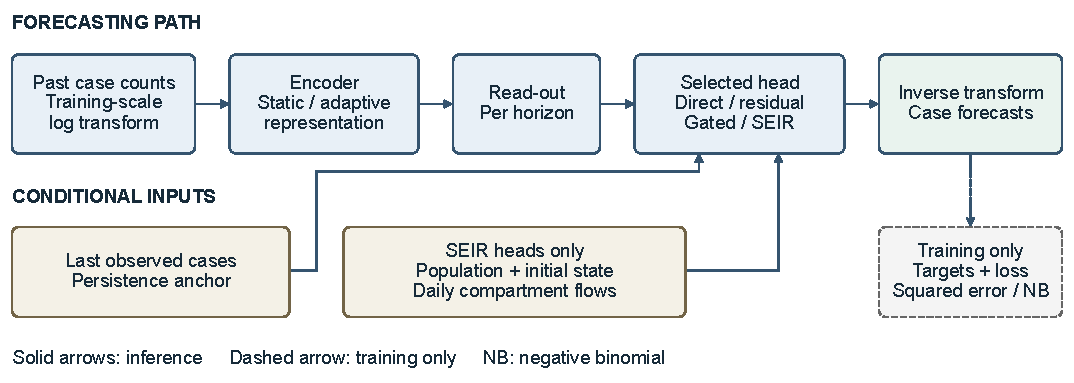
\includegraphics[width=\textwidth]{figures/fig_arch.pdf}
\caption{Neural forecasting paths. The selected output head uses the read-out directly, adds a residual to persistence, or blends a direct or SEIR forecast with persistence. SEIR heads additionally use population and initial compartment fractions. Solid paths operate at inference; the dashed target/loss path operates only during training. NB denotes negative binomial.}
\label{fig:arch}
\end{figure*}

\subsection{Inputs and encoders}
We work with log counts standardized on the training weeks only,
\begin{equation}
z_{i,t}=\frac{\log(1+c_{i,t})-\mu}{\sigma},
\label{eq:z}
\end{equation}
% seirgnn2/core.py::build_tensors (z), build_folds (mu, sigma from training weeks)
where $c_{i,t}$ is the count in district $i$ and week $t$, and $\mu,\sigma$ are the mean and standard deviation of $\log(1+c)$ over the training weeks.
The persistence anchor $p_{i,h}$ is the standardized last observed week, repeated over the horizon.

Our own graph convolutional network (GCN) encoder projects the input window to 64 dimensions and applies two message-passing layers with a residual connection around each, % EV-177
\begin{equation}
H^{(l+1)}=H^{(l)}+\mathrm{Dropout}\!\left(\mathrm{ReLU}\!\left(A\,H^{(l)}W^{(l)}+b^{(l)}\right)\right).
\label{eq:layer}
\end{equation}
% seirgnn2/models.py::GraphLayer.forward, Net.encode
Here $A$ mixes each district with its neighbors.
For the GCN encoder $A$ is the row-normalized border adjacency with self-loops. % EV-183
For the adaptive encoder it is learned,
\begin{equation}
A_{\mathrm{ad}}=\mathrm{softmax}\!\left(\mathrm{ReLU}\!\left(E_1E_2^{\top}\right)\right),
\label{eq:adaptive}
\end{equation}
% seirgnn2/models.py::learned_adjacency
with node embeddings $E_1,E_2\in\mathbb{R}^{25\times 10}$ drawn from a standard normal distribution, shared by both layers and exempt from weight decay. % EV-177
A small initialization gives an almost uniform $A_{\mathrm{ad}}$, which is plain averaging over all districts, and weight decay pulls the embeddings back toward it; we therefore use the standard-normal draw and the exemption, and we did not ablate the exemption alone. % EV-050
We also use five published encoders, STGAT, A3T-GCN, ASTGCN, AAGCN and DCRNN, transcribed from the reference code and checked against it, and Liu et al.'s LSTM~\cite{weng2024graph,liu2025seirlstm}.
Our STGAT is the dengue adaptation in that code, a graph-attention layer followed by two LSTM layers, and not the original pedestrian model~\cite{huang2019stgat}.
They replace the graph layers and output a 64-dimensional representation per district.

\subsection{Output heads}
Let $r$ be a linear read-out of the representation.
The five heads are
\begin{equation}
\hat z=\begin{cases}
r & \text{direct}\\
p+r & \text{residual}\\
p+\sigma(a)\,(r-p) & \text{gated}\\
z(\hat c) & \text{SEIR}\\
p+\sigma(a)\,\bigl(z(\hat c)-p\bigr) & \text{gated SEIR}
\end{cases}
\label{eq:heads}
\end{equation}
% seirgnn2/models.py::Net.forward (direct, residual, gated, foi, foi_res)
where $a$ is a learned scalar initialized at $-2$ so that the gate starts mostly closed, % EV-178
and $z(\hat c)$ standardizes the SEIR count forecast $\hat c$ with Eq.~\eqref{eq:z}.
Here $\sigma(\cdot)$ denotes the sigmoid function.

\subsection{SEIR decoder}
For each district the decoder tracks the susceptible, exposed, infectious and recovered fractions $(S,E,I,R)$.
It steps one day at a time with exponential flows, using a force of infection $\lambda_{i,h}$ that is constant within forecast week $h$,
\begin{equation}
\begin{aligned}
f_S&=S\,(1-e^{-\lambda\Delta t}), & S&\leftarrow S-f_S,\\
f_E&=E\,(1-e^{-\omega\Delta t}), & E&\leftarrow E+f_S-f_E,\\
f_I&=I\,(1-e^{-\gamma\Delta t}), & I&\leftarrow I+f_E-f_I,
\end{aligned}
\label{eq:seir}
\end{equation}
% analysis/lib/seir_sim.py::_step, simulate_weeks (R <- R + f_I)
All flows are computed from the state before the daily update, and $R$ increases by $f_I$.
We use $\Delta t$ of one day, $\omega=0.7/7$ and $\gamma=1/7$ per day, and 7 steps per week. % EV-011
The weekly count forecast is $\hat c_{i,h}=\rho_{\rm eff} N_i\sum_{d=1}^{7}f_E^{(d)}$, where $N_i$ is the district population and the base reporting fraction is $\rho=1/11$; the learned effective fraction is defined below. % EV-011, EV-217
% seirgnn2/models.py::Net._physics (counts = inc * rho * pop)
The initial state comes from the last two reported weeks, with the infectious fraction set from $c_{t-1}/(\rho N_i)$ and the exposed fraction from $c_{t-2}/(\rho N_i)$. % EV-170
The susceptible fraction starts from $1-0.682$ and falls with cumulative cases scaled by reporting and population~\cite{jeewandara2015sero}. % EV-170
Compartment fractions are clipped as implemented in the initial-state function.
The exposed fraction and the reporting fraction each carry one learned multiplier; for one variant the exposed multiplier is a function of the district encoding. % EV-173
In heads with state fitting, the effective reporting fraction is $\rho_{\rm eff}=\rho\exp(q)$, with learned scalar $q$.
The exposed fraction is multiplied by twice a sigmoid, predicted globally or from the encoding.
The removed or added exposed mass is compensated in the recovered compartment, subject to clipping.
% seirgnn2/models.py::Net._seed and Net._physics

We test two ways to form the force of infection from the read-out $r$.
The free rate exponentiates $r+b$ after lower and upper clipping, with learned bias $b$. % EV-171
The free rate must therefore learn an offset of about $-\log(\rho N_i S)$ for each district, although it never sees population or $S$.
The anchored rate supplies that scale,
\begin{equation}
\begin{aligned}
\hat\lambda_i&=\frac{\max\!\left(c_{i,t-1},\,0.5\right)}{7\,\rho_{\rm eff}\,N_i\,S_i},\\
\lambda^*_{i,h}&=\hat\lambda_i\exp\!\bigl(\mathrm{clip}(r_{i,h},-10,10)\bigr).
\end{aligned}
\label{eq:anchor}
\end{equation}
% seirgnn2/models.py::Net._physics, lam_param == "anchor", l.351-358
The first term approximates the daily rate needed to sustain the latest count, ignoring depletion and latent progression.
The second lets the network increase or decrease that rate.
At $r=0$ the SEIR forecast is close to last week's count but not equal to it, because the simulator does not start in equilibrium, and $S_i$ is the susceptible fraction at the forecast origin.
The simulator additionally applies a learned spatial-import factor,
\begin{equation}
u_i=\log\max\bigl((A I)_i,10^{-9}\bigr),\quad
\lambda_{i,h}=\lambda^*_{i,h}\exp\bigl(0.1\beta(u_i-\bar u)\bigr),
\end{equation}
% seirgnn2/models.py::Net._physics, lines 363-370; EV-217
where $\bar u$ is the district mean within the same window and $\beta$ is learned.
The same factor multiplies the free-rate head; it uses the fixed adjacency, including in adaptive-encoder runs.
Count conversion also uses $\rho_{\rm eff}$ when state fitting is enabled.
The mass-action variant instead predicts a positive transmission coefficient per forecast week and sets the daily rate to that coefficient times the current infectious fraction.
The simulator updates this fraction each day; this variant omits the spatial-import factor above.
% seirgnn2/models.py::Net._physics lam_param == "mass"; analysis/lib/seir_sim.py::simulate_closed_loop

\subsection{Loss, likelihood and training}
The default loss is squared error between $\hat z$ and the standardized target.
Squared error targets the conditional mean on the transformed scale.
Exponentiating that mean generally does not recover the conditional mean count, which minimizes count-scale squared error.
Auxiliary historical experiments also used a negative-binomial count likelihood; those results are excluded here pending corrected-data reruns.

All models use Adam with a learning rate of 3e-3 and weight decay of 1e-4, batches of 32, cosine learning-rate decay, gradient clipping at 5, and 300 epochs (400 with the NB loss). % EV-175
Early stopping watches validation RMSE in counts with a patience of 40 epochs and restores the best weights. % EV-175
The nine-origin encoders use case histories; their SEIR heads additionally use population and initial states. % EV-179, EV-170

%=====================================================================
\section{Experimental Setup}\label{sec:setup}
\subsection{Rolling-origin evaluation}
We use rolling-origin cross-validation: we train on all weeks before a cut-off date, test on the weeks after it, then move the cut-off forward and repeat.
For an origin $o$, the cut-off is at a fraction $o$ of all forecast windows.
The 30 forecast starts before the cut-off define validation; the next block defines test starts before missing-window filtering. % EV-182
Standardization uses the training-period history, partitions follow forecast-start chronology, and windows that touch a missing week are removed.
Training windows are randomly permuted into minibatches within the training partition.
The implemented split has two shared target weeks at each training/validation and validation/test boundary because adjacent forecasts overlap. % EV-218
This permits early stopping to use targets also present in the first test forecasts and prevents a strictly held-out interpretation.
The historical development protocol has nine origins from 0.50 to 0.90 in steps of 0.05, and each test block is 5\% of the windows. % EV-186, EV-141
We also use a three-origin protocol (0.55, 0.70, 0.85, test blocks of 15\%) for the wider ablation, because it needs fewer runs. % EV-186, EV-141
Every configuration is trained with seeds 0, 1 and 2 at every origin, which gives 27 runs per arm in the main protocol and 9 in the three-origin protocol. % EV-101, EV-116
The supplementary three-origin results use different test periods and are not compared with the nine-origin table.

\begin{figure}[t]
\centering
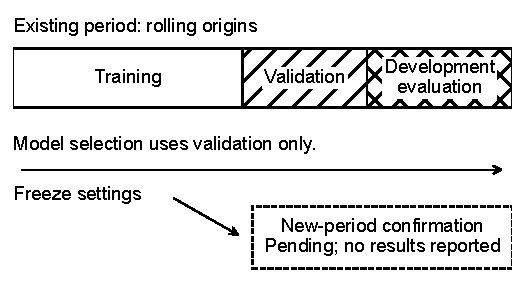
\includegraphics[width=\columnwidth]{figures/evaluation_protocol.pdf}
\caption{Evaluation chronology of forecast starts. Existing-period origins contain training, validation, and development evaluation, but their forecast targets overlap at partition boundaries. Freezing selected settings precedes new-period confirmation. The dashed box is planned, with no result available. Positions are schematic rather than proportional to elapsed time.}
\label{fig:protocol}
\end{figure}


\subsection{Baselines, selection and tests}
Persistence is the first baseline, reported at every horizon.
The baseline GNN is a GCN encoder with a residual head on log counts, which predicts a correction to persistence.
It follows the design of our first tuned baseline, which matched persistence where a GCN trained on absolute counts lost to it, and we retrain it here under the new protocol. % EV-191
Early stopping uses validation RMSE.
However, earlier evaluations had exposed these test weeks before later arms were chosen, so the stored comparisons are development evidence.
No untouched-period confirmatory result is reported here.
We compare each arm with persistence using the exact paired sign-flip test on the nine origin means, with seeds averaged within each origin, and adjust $p$-values over all 30 arms with the Benjamini-Hochberg procedure. % EV-149
With three origins, the smallest attainable $p$ is 0.25, so three-origin gaps are reported but not tested; with nine origins it is 0.0039. % EV-181
We do not pool seeds as independent evidence, because the three seeds at one origin share the same data.

The 30 arms of the main protocol are 24 arms from a full grid of six encoders (GCN, LSTM, STGAT, A3T-GCN, ASTGCN, AAGCN) and four heads (direct, residual, SEIR with a free rate, gated SEIR with a free rate), and 6 arms chosen by hand. % EV-179
One author chose the six hand-picked arms after the earlier results were known, and they were not registered in advance. % EV-184
They are five adaptive-encoder variants (a residual head, two anchored gated SEIR heads, an anchored bare SEIR head, a mass-action head) and the GCN encoder with the anchored gated head.
We report all of them next to the 24 grid arms and correct over all 30, but their selection is a weakness that we return to in Section~\ref{sec:discussion}.

%=====================================================================
\section{Results}\label{sec:results}
\subsection{Historical development results}
\begin{table*}[t]
\centering
\caption{Test results on the rebuilt series (nine rolling origins, three seeds). RMSE and MAE are in cases per district-week, averaged over origins and seeds; horizon columns report RMSE. $\Delta$ is the seed-averaged paired RMSE difference from persistence with a 95\% t interval over origins (negative is better). $p_{\rm adj}$ is the exact sign-flip test with Holm adjustment over all thirty learned arms. Bold marks the lowest test RMSE (the proposed Adaptive SEIR-GNN); no difference is significant after adjustment.}
\label{tab:main}
\small\setlength{\tabcolsep}{3pt}
\begin{tabular}{@{}p{2.85in}rrrrrr@{}}
\toprule
Model & $h=1$ & $h=2$ & $h=3$ & RMSE & MAE & $\Delta$ [95\% CI]; $p_{\rm adj}$ \\
\midrule
Persistence (last week) & 23.47 & 27.94 & 33.26 & 28.54 & 13.94 & -- \\ % EV-200

GCN, direct & 23.10 & 27.82 & 32.68 & 28.17 & 13.66 & -0.37 [-1.88, +1.14]; 1.000 \\ % EV-201

GCN, residual (baseline GNN) & 23.24 & 27.79 & 32.47 & 28.12 & 13.62 & -0.42 [-1.54, +0.70]; 1.000 \\ % EV-202

LSTM, direct & 23.65 & 28.22 & 33.38 & 28.73 & 14.00 & +0.19 [-1.99, +2.37]; 1.000 \\ % EV-203

ASTGCN, direct & 23.92 & 28.54 & 33.45 & 28.94 & 14.27 & +0.40 [-2.02, +2.81]; 1.000 \\ % EV-204

AAGCN, direct & 24.11 & 29.10 & 33.66 & 29.26 & 14.06 & +0.72 [-1.57, +3.00]; 1.000 \\ % EV-205

STGAT, direct & 42.60 & 44.55 & 46.75 & 44.71 & 22.17 & +16.17 [+4.24, +28.11]; 0.227 \\ % EV-206

ASTGCN, residual & 23.07 & 28.08 & 33.66 & 28.65 & 13.98 & +0.11 [-1.68, +1.90]; 1.000 \\ % EV-207

Adaptive GCN, residual & 23.07 & 27.78 & 32.15 & 27.94 & 13.61 & -0.60 [-1.81, +0.61]; 1.000 \\ % EV-208

GCN, SEIR, free rate & 27.58 & 40.81 & 50.14 & 40.77 & 17.97 & +12.23 [+2.67, +21.80]; 0.227 \\ % EV-209

GCN, gated SEIR, free rate & 22.86 & 28.04 & 33.29 & 28.43 & 13.51 & -0.11 [-3.23, +3.00]; 1.000 \\ % EV-210

Adaptive GCN, SEIR, anchored & 23.99 & 28.81 & 35.29 & 29.80 & 13.84 & +1.26 [-1.47, +3.98]; 1.000 \\ % EV-211

Adaptive GCN, gated SEIR, mass-action & 22.90 & 28.02 & 33.19 & 28.39 & 13.52 & -0.16 [-3.16, +2.85]; 1.000 \\ % EV-212

GCN, gated SEIR, anchored & 22.49 & 27.38 & 32.04 & 27.62 & 13.39 & -0.92 [-2.60, +0.76]; 1.000 \\ % EV-213

Adaptive GCN, gated SEIR, anchored & 22.51 & 27.09 & 31.85 & 27.45 & 13.31 & -1.09 [-2.81, +0.63]; 1.000 \\ % EV-214

\textbf{Adaptive GCN, gated SEIR, anchored, learned $E_0$} & \textbf{22.45} & \textbf{27.07} & \textbf{31.88} & \textbf{27.45} & \textbf{13.29} & \textbf{-1.10 [-2.84, +0.65]; 1.000} \\ % EV-215

\bottomrule
\end{tabular}
\end{table*}


Table~\ref{tab:main} compares selected stored arms with persistence on the historical nine-origin protocol.
Fig.~\ref{fig:forest} shows paired uncertainty for the baseline and anchored variants.
These are development comparisons using the original graph, not corrected-graph or untouched-period results.
No learned arm is significantly better than persistence on test, and eight are significantly worse. % EV-150
The lowest test RMSE is 27.45, against 28.54 for persistence, shared by the two anchored gated SEIR arms with an adaptive graph (adjusted $p$ is 0.576). % EV-100, EV-113, EV-114
The baseline GNN, a GCN with a residual head, scores 28.12, which is 0.42 below persistence (adjusted $p$ of 0.781). % EV-102
At the three horizons it is lower than persistence by 0.23, 0.15 and 0.79 cases. % EV-165
The same encoder with a direct head scores 28.17 (adjusted $p$ of 0.984). % EV-101
The anchored gated SEIR arm with an adaptive graph is lower than persistence by 0.97, 0.85 and 1.41 cases, so the gap grows with the horizon, but it stays small beside a persistence RMSE of 33.26 at $h=3$. % EV-152, EV-100
STGAT with a direct head has an RMSE of 44.71 under the shared fixed training settings. % EV-106


Validation tells a different story.
On validation, seven arms are significantly better than persistence and eight are significantly worse. % EV-149
One of the seven is the adaptive encoder with a residual head, with a validation RMSE of 25.42 against 27.04 for persistence and an adjusted $p$ of 0.023. % EV-108, EV-100
On test the same model scores 27.94 against 28.54, a gap of 0.60 with an adjusted $p$ of 0.694. % EV-108, EV-100
Selecting on validation would have reported a significant gain that the test blocks do not support.

\begin{figure}[t]
\centering
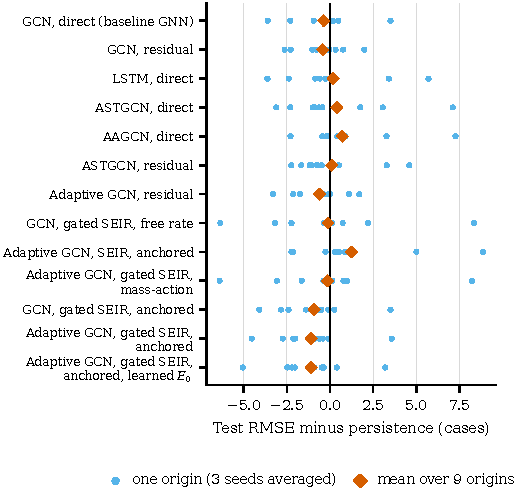
\includegraphics[width=\columnwidth]{figures/fig_forest.pdf}
\caption{Selected historical development comparisons against persistence. Points are mean paired test RMSE differences after averaging seeds within each origin; bars are descriptive 95\% t intervals over the nine origins. The dashed line denotes no difference. Selection was retrospective, temporal dependence limits inference, and the intervals are not multiplicity-adjusted.}
\label{fig:forest}
\end{figure}

\subsection{The SEIR head and its parameterization}
With a free rate, the bare SEIR head on a GCN scores 40.77, which is 12.23 cases worse than persistence (adjusted $p$ of 0.033). % EV-109
With the anchored rate and an adaptive graph, the bare head scores 29.80, which is 1.26 cases worse and not significant (adjusted $p$ of 0.781). % EV-111
These two arms differ in the graph as well as in the rate, so the change cannot be assigned to the rate alone.
We have no bare-head arm that pairs the two rates on one graph.
For the gated head the pairing exists: on a GCN encoder, the anchored rate gives 27.62 and the free rate gives 28.43, and neither is significantly different from persistence. % EV-112, EV-110

The supplementary material reports the historical three-origin encoder/head ablation separately.
Its test blocks differ from the nine-origin evaluation, so their scores are not compared.
With three origins no exact sign-flip test can reach $p$ below 0.25. % EV-181
In that exploratory comparison, gated SEIR heads have lower test error than matched gated heads without a simulator, while validation differences are mixed. % EV-159, EV-160, EV-161
Equal validation-only tuning and the corresponding adaptive-encoder controls are missing.
The results therefore do not isolate a predictive benefit from the epidemic equations.

\subsection{Results awaiting corrected-data reruns}
The seasonal, climate, and policy comparisons used date-joined inputs affected by errors in the historical calendar.
Those results are excluded from the present claims while replacement runs are pending.
The associated model-B negative-ablation table and validation/test scatter are omitted for the same reason.
We retain their source scripts and archived outputs for traceability.
Classical baselines, equal-budget tuning, and the missing adaptive-encoder ablations also remain outstanding.

Older legacy-array tests are exploratory and cannot be compared with Table~\ref{tab:main}.
WGAN-GP augmentation raised RMSE on the middle fold to 124.13, against 43.71 without augmentation and 41.74 with jitter and warping. % EV-086
This single-fold historical result supports neither a general claim about augmentation nor a contribution of the final architecture.

\subsection{Historical interval comparison}
On legacy-array folds containing the source-table error, residual-based persistence intervals have similar coverage and smaller mean widths than the Gaussian-head intervals.
The supplementary material reports coverage together with width; this historical result is not a calibration contribution.


%=====================================================================
\section{Discussion and Limitations}\label{sec:discussion}
\subsection{What we learned}
Persistence is competitive on the stored development comparisons.
Strong pooled lagged association motivates this baseline, but it does not bound the variance a forecast can explain.
Large districts and outbreak weeks can influence pooled correlations.
The direct-head models received shared fixed training settings rather than equal validation-only tuning.
Their high errors therefore do not establish that the underlying encoder architectures are unsuitable for dengue.
The gated-head comparison also differs between validation and test.
We cannot attribute the validation repair to the epidemic equations, or generalize this result to epidemic models as a class.

A log-only force-of-infection diagnostic suggests both an unobserved scale offset and an exposed-compartment floor.
This diagnostic is not a trained-head comparison and remains to be archived as a saved output.

The learned adjacency does move away from uniform: its normalized row entropy is 0.469 on average, against 1.000 for a uniform matrix. % EV-050
Its strongest edges do not follow geography.
Examples are Kalutara from Kandy and Jaffna from Kegalle, which are not neighbors. % EV-185
These weights have not been validated as transmission pathways.
A numerical difference from the no-graph control on the three-origin protocol is descriptive only. % EV-117, EV-118, EV-116

Among the displayed arms, ASTGCN with a residual head has the lowest validation RMSE, 25.23, and is 0.11 above persistence on test. % EV-107

\subsection{Limitations}
The nine origins give 9 paired units, which allows $p$ down to 0.0039; precision remains limited. % EV-181
Six of the 30 main arms were hand-picked after earlier results, the 46-arm grid planned for them was not run, and the Benjamini-Hochberg family therefore does not describe a clean selection. % EV-184
The static graph in all main runs contains two edges that are not real borders, Kandy to Ampara and Kegalle to Kalutara; a corrected file exists, and we did not repeat the main runs with it. % EV-010
The latent and infectious rates are fixed; learned multipliers modify reporting and the exposed initial state in selected heads. % EV-011
The interval comparison and the older WGAN-GP and adaptive-graph results use the legacy array, which contains the week-395 error. % EV-162
Serial dependence between rolling-origin scores and retrospective selection limit the descriptive intervals and paired tests.
A non-significant difference is not evidence of equivalence.
Population-vintage and NDVI-availability rules have since changed; stored scores must not be described as using those later rules.
The latest evaluation design requires a constant Census population and explicit treatment of irregular report lengths and missing inputs.
That design remains pending, as Fig.~\ref{fig:protocol} indicates.
We study one country, one disease and a horizon of three weeks.

%=====================================================================
\section{Conclusion}
The stored development evaluation shows that persistence is competitive with the tested graph and SEIR-head variants.
The lowest stored learned-model RMSE is 27.45, compared with 28.54 for persistence, but the paired interval includes zero and the adjusted test value is 0.576. % EV-100, EV-114, EV-215
Mixed validation/test results and missing matched controls prevent attributing an accuracy gain to the epidemic equations.
Corrected-data reruns, fair tuning, classical baselines, and the untouched-period evaluation are required before a confirmatory conclusion.

\section*{Acknowledgment}
% TODO(authors): add funding or supervisor acknowledgment only if applicable.
AI use: Claude Code assisted with repository analysis and drafting; Codex assisted with source checks, figure generation, and manuscript revision.
% TODO(authors): verify this account of tool use and independently approve all claims before submission.
Author verification and approval remain pending.

\bibliographystyle{IEEEtran}
\bibliography{refs}

\end{document}
